\section{\tool}
\label{sec:badusb}
\subsection{Motivation}
\noindent\outline{Limitation of Rubber Ducky}\\
\outline{Our functionality different mode listing?}\\
\hongyi{The following mode is to be further decided}
\outline{Automatic Scripting Mode}\\
\outline{Remote Control Mode}\\
\outline{OCR/QR Recognition Mode}\\
As we introduced in the Section~\ref{sec:related_work}, there are plenty of existing work \shuqing{Add citation} focusing on BadUSB attack. 
Many of these take use of the \textit{default trust} given by computers to HIDs, pretend normal USB devices as HIDs and uitilize USB protocol to perform attacks. 
However, these attacks suffer from various drawbacks:
\ding{182} attackers can only simulate limited types of HIDs like keyboards, mice, and disks, which makes the attacks less effective;
\ding{183} accurate attacks couldn't be performed due to lacking of user interface (UI).
Whatever HID the attackers simulate their USB devices to be, they couldn't obtain the UI to check the current situation, which makes it nearly impossible to locate their attacks precisely or confirm the effects after attacks.

In this work, we utilized the new features of USB-C to address the problems above.
Benefiting from USB-C, we simulated vedio card and thus obtained the video stream of UI to perform accurate attacks.

\subsection{Implementation}
\noindent\hongyi{The following mode is to be further decided}\\
\outline{DETAIL of each mode}\\
\outline{Automatic Scripting Mode}\\
\outline{Remote Control Mode}\\
\outline{OCR/QR Recognition Mode}\\
The implementation of \tool\ extends several existing offensive BadUSB device including Rubber Ducky\hongyi{Add Citation} (where we implement the co-operation of HID emulation and screen streaming) and Raspberry Pi (on which we implement the capture of video stream and its processing). We implemented the QR-Code extraction agent from scratch. The complete workflow of \tool, demonstrating the interaction of all the components is presented at Fig.~\ref{fig:workflow}.

\begin{figure}[htbp]
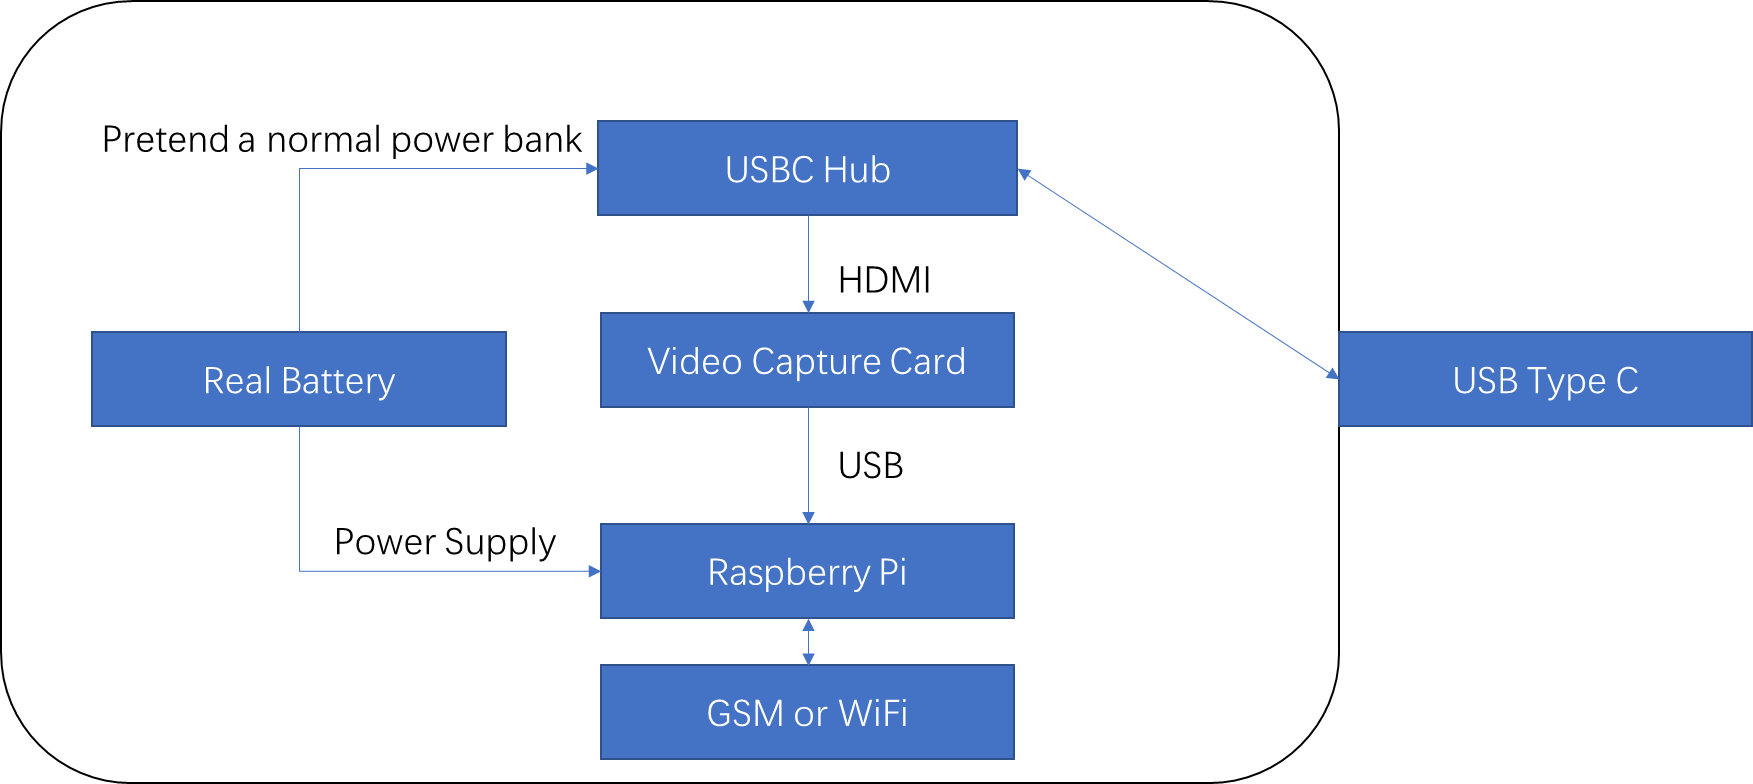
\includegraphics[width=\linewidth]{./Figs/workflow.png}
\caption{Workflow of \tool}
\label{fig:workflow}
\end{figure}

When the victim plugs in \tool device, the USB-C hub handles all the communication between each components and the victim's device. Due to the trust-by-default feature of USB protocol, the victim's video stream will be captured. Later, the stream is either processed directly by Raspberry Pi or transmitted to the attacker through GSM/WiFi components.

With video stream the capability of original Rubbery Ducky attack is considerably expanded. For example, the attacker can directly control the victim's device and view the private data in the stream. More details is presented in the Section~\ref{sec:experiment}